\documentclass[10pt,a4paper]{article}
\usepackage[margin=2.2cm]{geometry}
\usepackage{fontspec}
\usepackage{kotex}
\setmainfont{Apple SD Gothic Neo}
\setsansfont{Apple SD Gothic Neo}
\usepackage{amsmath,amssymb}
\usepackage{graphicx}
\usepackage{booktabs}
\usepackage{caption}
\usepackage[dvipsnames]{xcolor}
\usepackage[colorlinks=true,linkcolor=MidnightBlue,citecolor=MidnightBlue,
            urlcolor=MidnightBlue]{hyperref}
\usepackage{titlesec}
\titleformat{\section}{\large\bfseries}{\thesection}{0.6em}{}
\titleformat{\subsection}{\normalsize\bfseries}{\thesubsection}{0.5em}{}
\captionsetup{font=small,labelfont=bf}
\setlength{\parskip}{0.35em}
\setlength{\parindent}{0pt}

\usepackage{mdframed}
\newmdenv[linewidth=0.4pt,linecolor=gray!60,backgroundcolor=gray!5,
          innertopmargin=6pt,innerbottommargin=6pt,skipabove=8pt,skipbelow=8pt]{claimbox}
\newcommand{\claim}[2]{\begin{claimbox}\textbf{주장.} #1\par\smallskip
  \textcolor{gray!70}{\textbf{반증 조건.} #2}\end{claimbox}}

\title{\bfseries 다섯 중 하나만 살아남았다\\[2pt]
\large 용량 곡선은 진단이고 처방이 아니다}
\author{월드모델 실험실 · 노트 678}
\date{2026-08-06}
\begin{document}\maketitle

\section{한 줄}

노트 675 가 \textbf{겹침 $\leftrightarrow$ 신호 몫 스피어만 $-1.000$} 을 쟀다. 그
곡선이 가리키는 처방은 명백했다 --- 겹침이 낮은 두 도메인에만 축을 붙여라. 단일
전환으로 재니 \textbf{하나는 부호가 뒤집히고}(만화 $+0.0184 \to -0.0027$)
\textbf{하나는 버텼다}(세계애니 $+0.0041 \to +0.0035$, 85\% 보존). 사전등록 규칙대로
\textbf{처방을 버린다.}

\section{왜 이걸 했나 --- 세 번 밟은 조항}

노트 551 · 560 · 563 이 같은 것을 세 번 쟀다: \emph{전역 변경의 도메인별 차로
후보를 세우면 그 도메인만 바꿀 때 부호가 뒤집힌다}(도서 $+0.0459 \to
\mathbf{-0.0820}$ · 게임 $-0.0137 \to \mathbf{+0.0138}$).

그런데 이번은 앞선 셋과 다른 점이 하나 있다고 봤다. 그때는 도메인을 \textbf{결과를
보고} 골랐고, 이번에는 \textbf{사전 예측자}가 있다 --- 겹침은 라벨을 안 보고
계산된다. 그래서 이 실험은 \emph{고르기}가 아니라 \emph{예측}이라고 사전등록에 적고,
판정 둘을 따로 못박았다: \textbf{(가)} 부호가 유지되나 \textbf{(나)} 판 문턱을 넘나.

\section{쟀다}

\begin{center}
\begin{tabular}{lrrr}
\toprule
팔 (만화 · 세계애니만) & 판 & 차 & 양수 \\
\midrule
① 없이 & 0.4689 & --- & --- \\
② 진짜 & 0.4683 & $-0.0005$ & 5/12 \\
③ 위약 & 0.4690 & $+0.0001$ & 6/12 \\
\bottomrule
\end{tabular}
\end{center}

판 신호 몫 $\mathbf{-0.0006}$, 문턱 $0.0045$. \textbf{(나) 미달} --- 사전등록 기대값이
$+0.0018$ 이었으니 예측대로다. 배선을 찍었고 관문 ③ 값이 전역 팔과 \textbf{동일}
($0.316$ · $0.403$)이라 축 정의는 안 바뀌었다(풀을 안 줄였다).

\begin{figure}[t]\centering
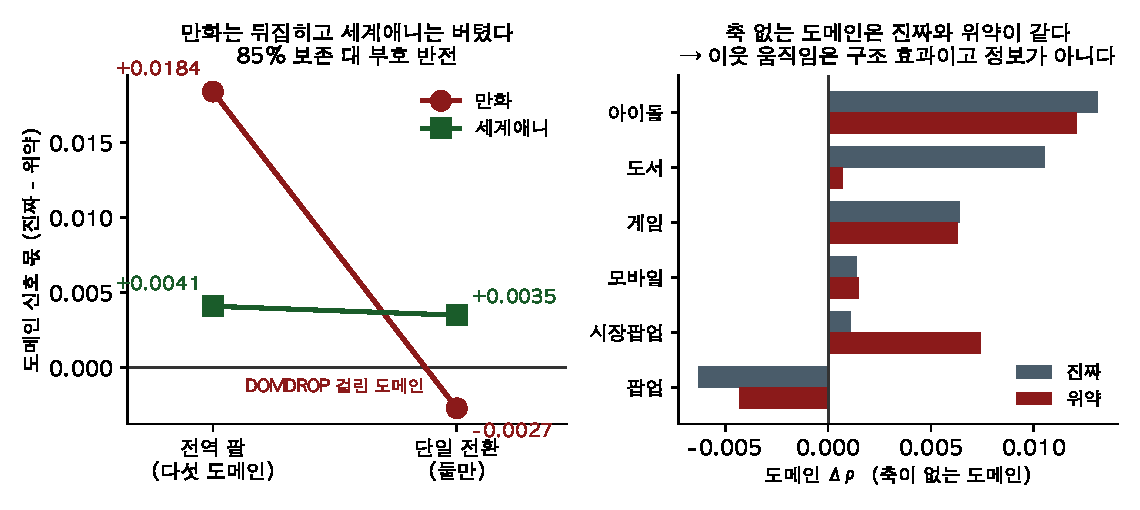
\includegraphics[width=0.99\textwidth]{figs/onesurvives.pdf}
\caption{왼쪽: \textbf{(가)} 도메인 신호 몫이 전역 팔에서 단일 전환으로 갈 때. 만화는
부호가 뒤집히고 세계애니는 부호와 크기를 다 지킨다. 오른쪽: 축이 \emph{없는} 도메인들이
진짜와 위약에서 거의 같게 움직인다(아이돌 $+0.0131$ 대 $+0.0121$ · 게임 $+0.0064$ 대
$+0.0063$ · 모바일 $+0.0014$ 대 $+0.0015$).}
\end{figure}

\claim{\textbf{(가)② 발동 --- 노트 551 · 560 · 563 조항이 네 번째로 확인됐다.}
겹침은 라벨을 안 보지만, \textbf{그 겹침이 예측하는 신호 몫은 다른 도메인이 무엇을
보는지에 달렸다.} 그래서 사전 예측자가 있어도 전역 표는 처방이 못 된다.}
{두 도메인이 다 부호를 지켰다면 조항에 예외가 하나 생겼을 것이다. 실제로 \emph{하나는}
지켰으므로 이 주장은 ``전역 표는 언제나 뒤집힌다''가 아니라 \textbf{``뒤집힐 수 있으므로
처방으로 쓸 수 없다''} 다.}

\section{그런데 하나는 버텼고, 그 차이를 미리 적어 뒀다}

사전등록 사각 ①에 이렇게 적었다: \emph{``만화는
\texttt{DOMDROP=\{"만화":("trend\_",)\}} 로 검색 축이 막혀 있다. 축 구성이 다른
도메인이므로 혼잡도 축이 상대적으로 더 크게 보일 수 있다. 그 가능성을 결과에
적는다.''}

\textbf{전역 팔에서 만화가 다섯 중 제일 컸던 것($+0.0184$)이 바로 그 크게 보임이었을
수 있다.} 세계애니는 축 구성이 표준이고 부호와 크기를 다 지켰다.

\claim{\textbf{전역 표로 도메인을 고를 때 \texttt{DOMDROP} · \texttt{BLOCK} 이 걸린
도메인을 먼저 뺀다.} 그 도메인은 다른 축 집합을 보므로 새 축의 상대적 크기가 부푼다.
지금 걸린 것은 만화 · 애니이므로 후보는 세계애니 · 모바일 · 게임이고, 그중 신호 몫이
양수였던 것은 \textbf{세계애니 하나}다.}
{애니(같은 \texttt{DOMDROP})의 신호 몫은 전역 팔에서 $-0.0047$ 로 이미 음수였다 ---
즉 \texttt{DOMDROP} 이 항상 부풀리는 것은 아니다. 이 주장은 ``부풀 수 있다''이고
``항상 부푼다''가 아니다.}

\section{덤 --- 신호 몫은 이웃 효과에 강하다}

축이 \emph{없는} 도메인들이 움직였다. 아이돌은 $+0.0131$ 인데 이 축을 한 번도 받은
적이 없다. 노트 551 이 말한 이웃 효과다. 그런데 \textbf{위약에서도 $+0.0121$} 이다.

\claim{이웃 움직임은 \textbf{열 집합이 바뀐 구조 효과}이고 정보가 아니다. 위약이 같은
구조를 지니므로 \textbf{신호 몫을 취하면 이웃 효과가 상쇄된다.} 노트 551 조항에 붙는
처방: \textbf{도메인별 차를 볼 때는 진짜가 아니라 신호 몫을 본다.}}
{\textbf{충분조건은 아니다} --- 신호 몫으로 봤는데도 만화는 뒤집혔다. 이웃 효과를
없애는 것과 전역/단일 차이를 없애는 것은 다른 문제다.}

\section{그래서 용량 곡선은 무엇으로 남나}

\textbf{처방으로는 죽었고 진단으로는 아직 살아 있다.} 진단이라는 것은 ``판 신호 몫이
0 일 때 그것이 상쇄인지 무신호인지 가른다''는 쓸모다 --- 노트 675 가 실제로 그것을
했다. 다음 시험은 \textbf{세계애니 하나만 붙여 씨앗 40 으로 재는 것}이고, 기대 판
이득은 유보 가중 $300/3369$ 로 $+0.0003$ 이라 \textbf{채택 실험이 아니라 재현
실험}이다. 씨앗 40 에서도 같으면 \emph{``겹침 낮은 표준 도메인에서는 재현된다''}가
서고, 그때 곡선은 진단으로 확정된다.

\end{document}
